\subsection{AF relaying with end-to-end ARQ}

Given that $p_{e,i} = 0.1, i = \{1,2 \dots r+1\}$ and $\mu_{AF} = \mu_{MS} = 2$,
the arrival rates at each relay station and at the mobile station are:

\begin{align*}
  \lambda_1 &= \dfrac{\lambda}{(1-0.1)^{r+1}} = \lambda\ 0.9^{-r-1} \\
  \lambda_2 &= \lambda_1 (1-0.1) = \lambda\ 0.9^{-r} \\
  \lambda_3 &= \lambda_2 (1-0.1) = \lambda\ 0.9^{-r + 1} \\
  & \dots \\
  \lambda_{r+1} &= \lambda\ 0.9^{-1}
\end{align*}

Since (a) the entire network is stable when all queues are stable, (b) every
station is a M/M/1 system, and (c) such a system is considered to be stable
when $\rho = \dfrac{\lambda}{\mu} < 1$, then the network is stable if all of the
following inequalities hold:

\begin{align*}
  &\lambda\cdot 0.9^{-r-1} < 2 \\
  &\lambda\cdot 0.9^{-r} < 2 \\
  &\lambda\cdot 0.9^{-r + 1} < 2 \\
  & \dots \\
  &\lambda\cdot 0.9^{-1} < 2
\end{align*}

or

\begin{align*}
  &\lambda < 2\cdot 0.9^{r+1}\\
  &\lambda < 2\cdot 0.9^{r}\\
  &\lambda < 2\cdot 0.9^{r-1}\\
  & \dots \\
  &\lambda < 2\cdot 0.9^{1}
\end{align*}

From these conditions, since $r \geq 1$ and $0.9 < 1$, we can see that the most
restrictive condition is the first one, i.e. if the first one holds, then,
inevitably, all the following conditions will be true. Figure
\ref{fig:04_stability_region_af_e2e} plots function
$\lambda_{max}(r) = 2 \cdot 0.9^{r+1}$ for $1 \leq r \leq 8$. The stability
region is defined as the region where $\lambda_{} < \lambda_{max}(r)$.

\begin{figure}\centering
  % This file was created by matlab2tikz.
%
%The latest updates can be retrieved from
%  http://www.mathworks.com/matlabcentral/fileexchange/22022-matlab2tikz-matlab2tikz
%where you can also make suggestions and rate matlab2tikz.
%
\definecolor{mycolor1}{rgb}{0.00000,0.44700,0.74100}%
%
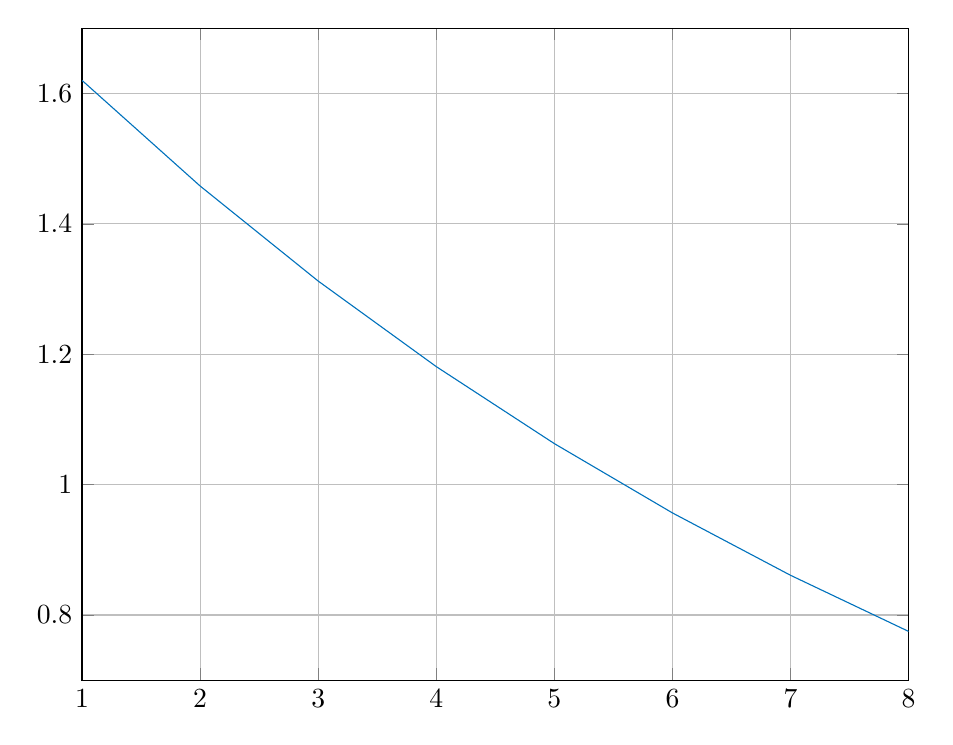
\begin{tikzpicture}

\begin{axis}[%
width=4.133in,
height=3.26in,
at={(0.693in,0.44in)},
scale only axis,
xmin=1,
xmax=8,
xmajorgrids,
ymin=0.7,
ymax=1.7,
ymajorgrids,
axis background/.style={fill=white}
]
\addplot [color=mycolor1,solid,forget plot]
  table[row sep=crcr]{%
1	1.62\\
2	1.458\\
3	1.3122\\
4	1.18098\\
5	1.062882\\
6	0.9565938\\
7	0.86093442\\
8	0.774840978\\
};
\end{axis}
\end{tikzpicture}%
  \caption{Function $\lambda_{max}(r) = 2\cdot 0.9^{r+1}$ for $1 \leq r \leq 8$.
    The stability region is the area under the curve.}
  \label{fig:04_stability_region_af_e2e}
\end{figure}

As $r \to \infty$, the stability region gets smaller and smaller in size, until
it is obliterated, since $\lambda_{max}(r) \to 0$ as $r \to \infty$.

This is reasonable, since, as $r$ increases, the number of relay stations
increase, and each one of them carries a probability of erroneous transmission
with it. Each erroneous packet has to be retransmitted from the base station,
and the end-to-end error probability goes to $1$ as $r \to \infty$:

\begin{align*}
  \displaystyle \lim_{r \to \infty} p_{e,e2e} = \lim_{r \to \infty} (1 - \prod\limits_{k=1}^{r+1} 0.9) = 1 - 0 = 1
\end{align*}


%-------------------------------------------------------------------------------
\subsection{DF relaying with end-to-end ARQ}

With $p_{e,i} = 0.1, i = \{1,2 \dots r+1\}$, the arrival rates at each relay
station and at the mobile station, given by equations \ref{eq:02_lambda_i}
and \ref{eq:02_lambda_r_plus_one}, become

\begin{align}
  \lambda_i = \dfrac{\lambda}{1 - \sum\limits_{k=0}^r \Big(0.1 \prod\limits_{i=1}^k (1 - 0.1)\Big)} \prod\limits_{k=1}^{i-1} (1 - 0.1)
  \label{eq:04_stability_region_df_e2e_lambda_i}
\end{align}

\begin{align}
  \lambda_{r+1} = \dfrac{\lambda}{1 - \sum\limits_{k=0}^r \Big(0.1 \prod\limits_{i=1}^k (1 - 0.1)\Big)} \prod\limits_{k=1}^{r} (1 - 0.1)
  \label{eq:04_stability_region_df_e2e_lambda_r_plus_one}
\end{align}

The first part of the right-hand side of the above 2 equations does not change
over each station, and is equal to

\begin{align*}
  \dfrac{\lambda}{1 - \sum\limits_{k=0}^r \Big(0.1 \prod\limits_{i=1}^k (1 - 0.1)\Big)} =
  \dfrac{\lambda}{1 - 0.1 \sum\limits_{k=0}^r 0.9^k} =
  \dfrac{\lambda}{1 - 0.1 \dfrac{1 - 0.9^{r+1}}{1- 0.9}} =
  \lambda \cdot 0.9^{-r-1}
\end{align*}

Hence, equations \ref{eq:04_stability_region_df_e2e_lambda_i} and
\ref{eq:04_stability_region_df_e2e_lambda_r_plus_one} become

\begin{align*}
  \lambda_i = \lambda \cdot 0.9^{-r-1} \prod\limits_{k=1}^{i-1} (1 - 0.1) = \lambda \cdot 0.9^{-r-1} \cdot 0.9^{i-1} = \lambda \cdot 0.9^{i-r-2}
\end{align*}

\begin{align*}
  \lambda_{r+1} = \lambda \cdot 0.9^{-r-1} \prod\limits_{k=1}^{r} (1 - 0.1) = \lambda \cdot 0.9^{-r-1} \cdot 0.9^r = \lambda \cdot 0.9^{-1}
\end{align*}

Since (a) the entire network is stable when all queues are stable, (b) every
station is a M/M/1 system, and (c) such a system is considered to be stable
when $\rho_k = \dfrac{\lambda_k}{\mu_k} < 1$, then, the network is stable if all
of the following inequalities hold:

\begin{align*}
  \lambda_i &< \mu_{DF} \\
  \lambda_{r+1} &< \mu_{MS} \\
\end{align*}

or

\begin{align*}
  \lambda &< 0.9^{r+1} \\
  \lambda &< 0.9^{r} \\
  \lambda &< 0.9^{+r-1} \\
  & \dots \\
  \lambda &< 0.9^2 \\
  \text{and}\\
  \lambda &< 2 \cdot 0.9
\end{align*}

From these conditions, since $r \geq 1$, we can see that the most
restrictive condition is the first one, i.e. if the first one holds, then,
inevitably, all the following conditions will be true. Figure
\ref{fig:04_stability_region_df_e2e} plots function
$\lambda_{max}(r) = 0.9^{r+1}$ for $1 \leq r \leq 8$. The stability
region is defined as the region where $\lambda_{} < \lambda_{max}(r)$.

\begin{figure}\centering
  % This file was created by matlab2tikz.
%
%The latest updates can be retrieved from
%  http://www.mathworks.com/matlabcentral/fileexchange/22022-matlab2tikz-matlab2tikz
%where you can also make suggestions and rate matlab2tikz.
%
\definecolor{mycolor1}{rgb}{0.00000,0.44700,0.74100}%
%
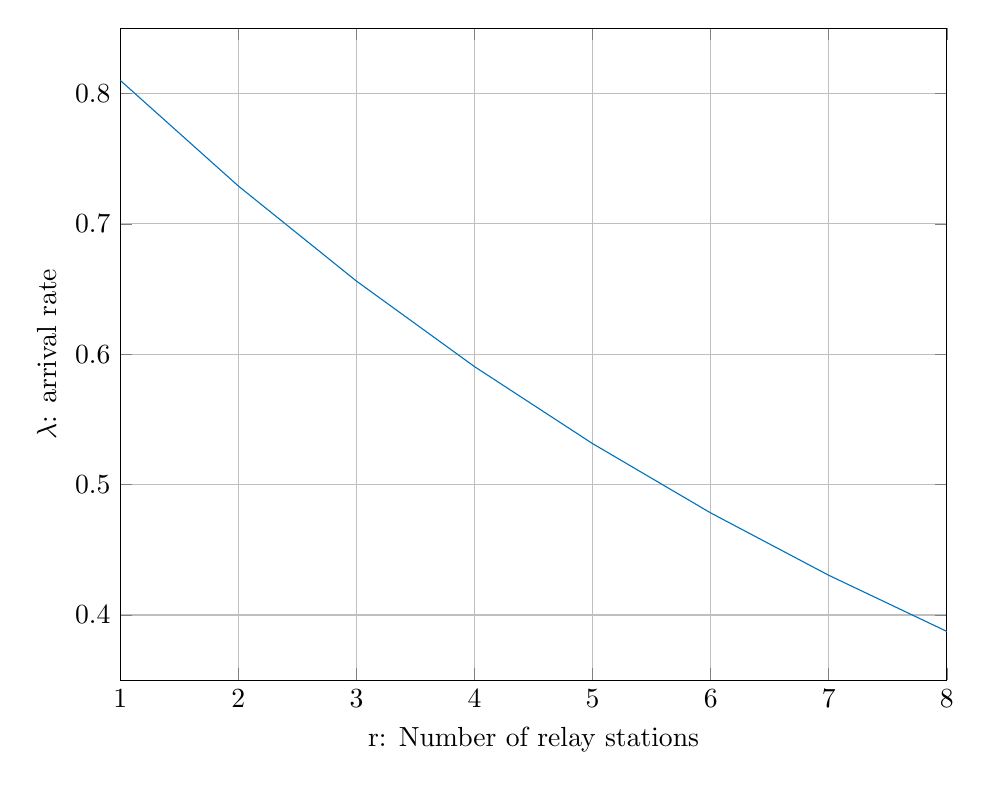
\begin{tikzpicture}

\begin{axis}[%
width=4.133in,
height=3.26in,
at={(0.693in,0.44in)},
scale only axis,
xmin=1,
xmax=8,
xmajorgrids,
xlabel={r: Number of relay stations},
ymin=0.35,
ymax=0.85,
ymajorgrids,
ylabel={$\lambda$: arrival rate},
axis background/.style={fill=white}
]
\addplot [color=mycolor1,solid,forget plot]
  table[row sep=crcr]{%
1	0.81\\
2	0.729\\
3	0.6561\\
4	0.59049\\
5	0.531441\\
6	0.4782969\\
7	0.43046721\\
8	0.387420489\\
};
\end{axis}
\end{tikzpicture}%

  \caption{Function $\lambda_{max}(r) = 0.9^{r+1}$ for $1 \leq r \leq 8$.
    The stability region is the area under the curve.}
  \label{fig:04_stability_region_df_e2e}
\end{figure}

As $r \to \infty$, the stability region gets smaller and smaller in size, until
it is obliterated, since $\lambda_{max}(r) \to 0$ as $r \to \infty$.

This is reasonable, since, as $r$ increases, the number of relay stations
increase, and each one of them carries a probability of erroneous transmission
with it. Each erroneous packet has to be retransmitted from the base station
and, hence, the load that the first relay station has to serve determines the
overall stability of the network.


%-------------------------------------------------------------------------------
\subsection{DF relaying with hop-by-hop ARQ}

With $p_{e,i} = 0.1, i = \{1,2 \dots r+1\}$, the arrival rates at each relay
station and at the mobile station, given by equations \ref{eq:03_lambda_i}
and \ref{eq:03_lambda_r_plus_one}, become

\begin{align}
  \lambda_i = \lambda \cdot 0.9^{-1}
  \label{eq:04_stability_region_df_hbh_lambda_i}
\end{align}

\begin{align}
  \lambda_{r+1} = \lambda \cdot 0.9^{-1}
  \label{eq:04_stability_region_df_hbh_lambda_r_plus_one}
\end{align}

Since (a) the entire network is stable when all queues are stable, (b) every
station is a M/M/1 system, and (c) such a system is considered to be stable
when $\rho_k = \dfrac{\lambda_k}{\mu_k} < 1$, then, the network is stable if all
of the following inequalities hold:

\begin{align*}
  &\lambda \cdot 0.9^{-1} < 1 \\
  &\lambda \cdot 0.9^{-1} < 2
\end{align*}

From these conditions  we can see that the most restrictive condition is the
first one, i.e. if the first one holds, then, inevitably, the second condition
will be true. Figure \ref{fig:04_stability_region_df_hbh} plots function
$\lambda_{max}(r) = 0.9$ for $1 \leq r \leq 8$. The stability
region is defined as the region where $\lambda_{} < \lambda_{max}(r)$.

\begin{figure}\centering
  % This file was created by matlab2tikz.
%
%The latest updates can be retrieved from
%  http://www.mathworks.com/matlabcentral/fileexchange/22022-matlab2tikz-matlab2tikz
%where you can also make suggestions and rate matlab2tikz.
%
\definecolor{mycolor1}{rgb}{0.00000,0.44700,0.74100}%
%
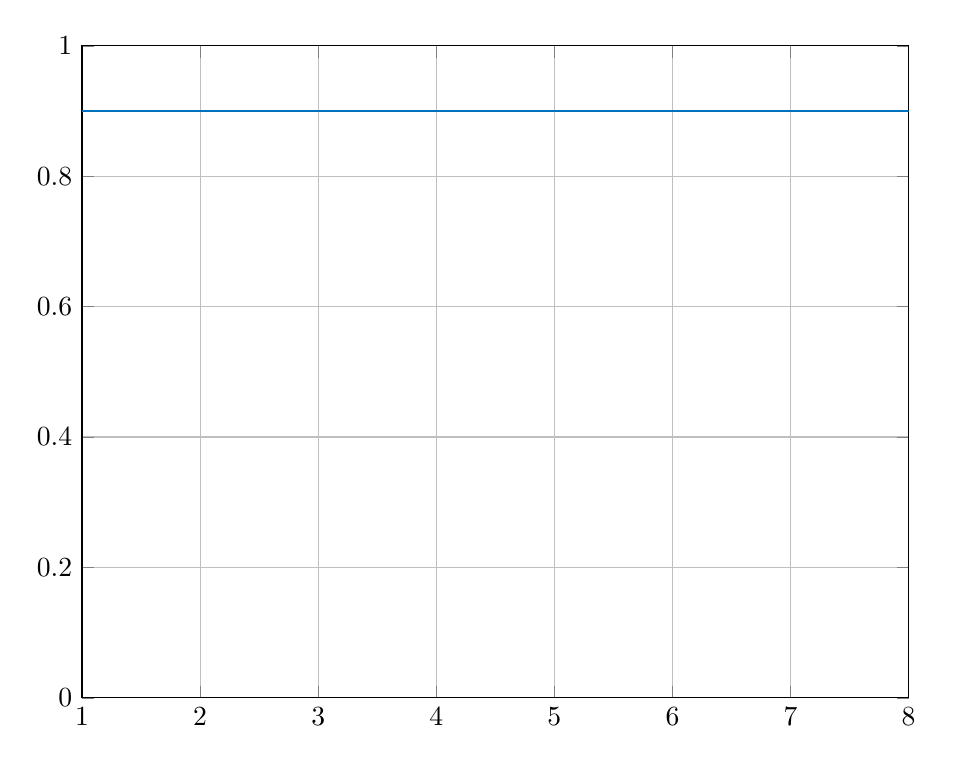
\begin{tikzpicture}

\begin{axis}[%
width=4.133in,
height=3.26in,
at={(0.693in,0.44in)},
scale only axis,
xmin=1,
xmax=8,
xmajorgrids,
ymin=0,
ymax=1,
ymajorgrids,
axis background/.style={fill=white}
]
\addplot [color=mycolor1,solid,forget plot]
  table[row sep=crcr]{%
1	0.9\\
2	0.9\\
3	0.9\\
4	0.9\\
5	0.9\\
6	0.9\\
7	0.9\\
8	0.9\\
};
\end{axis}
\end{tikzpicture}%
  \caption{Function $\lambda_{max}(r) = 0.9$ for $1 \leq r \leq 8$.
    The stability region is the area under the curve.}
  \label{fig:04_stability_region_df_hbh}
\end{figure}

As $r \to \infty$, the stability region is not affected.

This is reasonable, since, as $r$ increases, the number of relay stations
increase, and each one of them carries a probability of erroneous transmission
with it, but each erroneous packet doesn't have to be retransmitted from the
base station, as in the previous two networks, but from the station where the
error was made.

Figure \ref{fig:04_stability_regions} illustrates the maximum arrival rate
per queueing network for $1 \leq r \leq 8$.

\begin{figure}[H]\centering
  % This file was created by matlab2tikz.
%
%The latest updates can be retrieved from
%  http://www.mathworks.com/matlabcentral/fileexchange/22022-matlab2tikz-matlab2tikz
%where you can also make suggestions and rate matlab2tikz.
%
\definecolor{mycolor1}{rgb}{0.00000,0.44700,0.74100}%
\definecolor{mycolor2}{rgb}{0.85000,0.32500,0.09800}%
\definecolor{mycolor3}{rgb}{0.92900,0.69400,0.12500}%
%
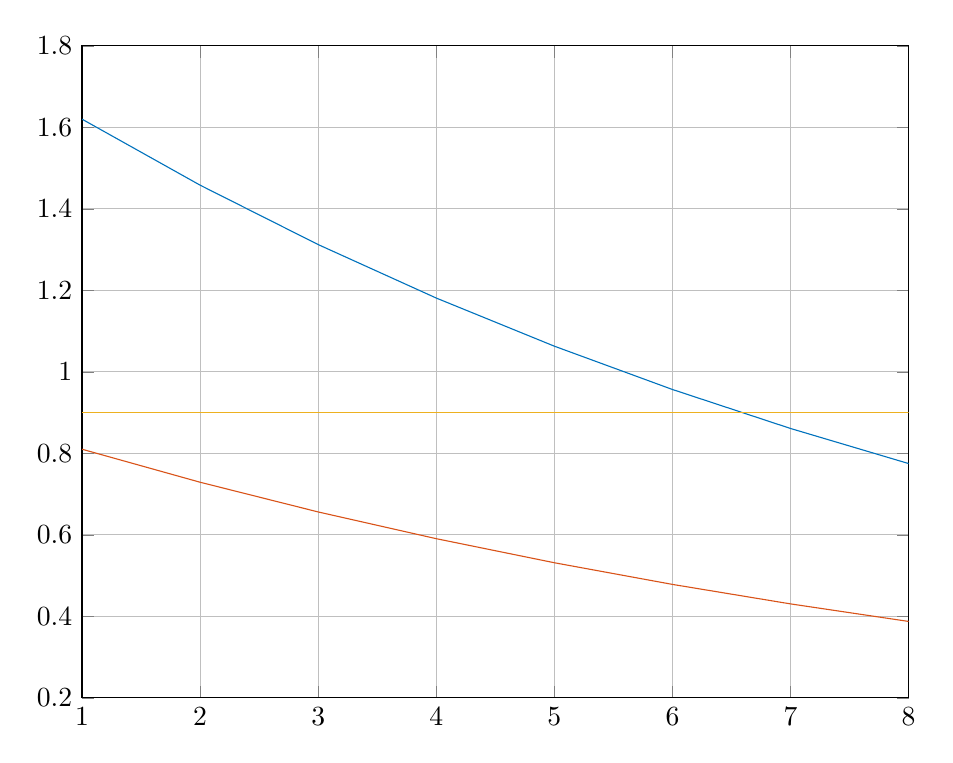
\begin{tikzpicture}

\begin{axis}[%
width=4.133in,
height=3.26in,
at={(0.693in,0.44in)},
scale only axis,
xmin=1,
xmax=8,
xmajorgrids,
ymin=0.2,
ymax=1.8,
ymajorgrids,
axis background/.style={fill=white}
]
\addplot [color=mycolor1,solid,forget plot]
  table[row sep=crcr]{%
1	1.62\\
2	1.458\\
3	1.3122\\
4	1.18098\\
5	1.062882\\
6	0.9565938\\
7	0.86093442\\
8	0.774840978\\
};
\addplot [color=mycolor2,solid,forget plot]
  table[row sep=crcr]{%
1	0.81\\
2	0.729\\
3	0.6561\\
4	0.59049\\
5	0.531441\\
6	0.4782969\\
7	0.43046721\\
8	0.387420489\\
};
\addplot [color=mycolor3,solid,forget plot]
  table[row sep=crcr]{%
1	0.9\\
2	0.9\\
3	0.9\\
4	0.9\\
5	0.9\\
6	0.9\\
7	0.9\\
8	0.9\\
};
\end{axis}
\end{tikzpicture}%
  \caption{The maximum arrival rate for each of the three queueing networks
    considered here, for $1 \leq r \leq 8$. Colour \texttt{blue} denotes that of
    AF with end-to-end ARQ, \texttt{red} that of DF with end-to-end ARQ and
    \texttt{orange} that of DF with hop-by-hop ARQ.}
  \label{fig:04_stability_regions}
\end{figure}
